\secrel{USB}\secdown

Использование одного из модулей USB интерфейса из библиотеки \odurino\ --- самый
простой и дешевый способ сделать из вашего компьютера или роутера простой 
контроллер для автоматизации какого-либо процесса, обработки сигналов с
датчиков, и прототирования алгоритмов управления.

Использование \termdef{bitbang}{bitbang} режимов микросхем usb-интерфейса
позволяет обойтись без использования микроконтроллера, и реализовать всю
програмную часть на компьютере. Это может быть полезным при отладке
(прототипировании) алгоритмов, а для коммерческих проектов позволяет обойтись
без специализированного программиста-ембедера (``железячника'').

\secrel{SparkFun/HEX FT232R Breakout}\label{HEXFT2232RL}

Модуль \href{https://www.sparkfun.com/products/retired/718}{SparkFun FT232R
Breakout} и подобные отличаются наличием полного набора выводов МС FTDI FT232R.
Такие модули удобны возможностью их использования в режиме FTDI BitBang как
универсальные программаторы для большого количества микроконтролеров, имеющих
последовательные интерфейсы программирования: SPI, UART BOOT0 и т.п.

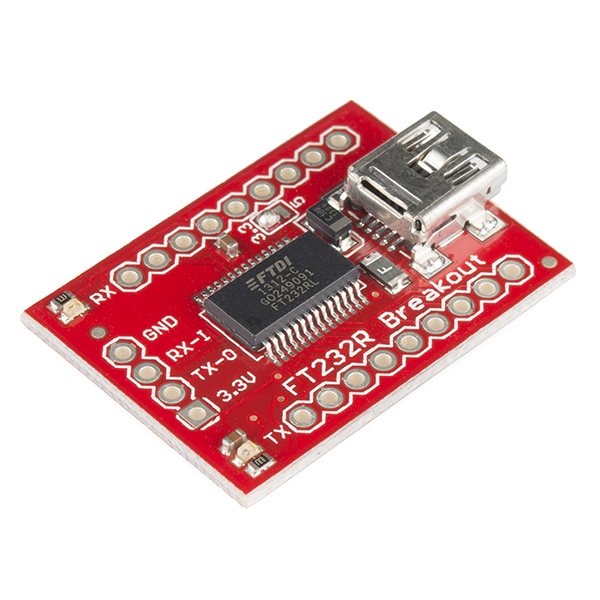
\includegraphics[width=0.3\textwidth]{odurino/usb/SF232R1.jpg}
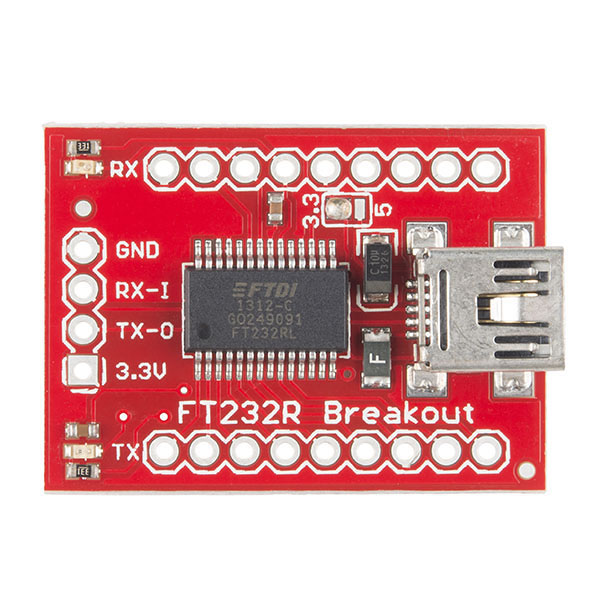
\includegraphics[width=0.3\textwidth]{odurino/usb/SF232R2.jpg}
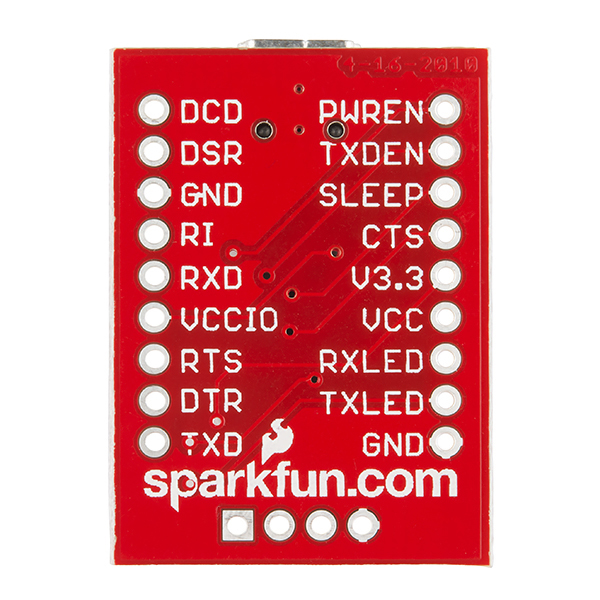
\includegraphics[width=0.3\textwidth]{odurino/usb/SF232R3.jpg}

\secup
